% GNUPLOT: LaTeX picture with Postscript
\begingroup
  \makeatletter
  \providecommand\color[2][]{%
    \GenericError{(gnuplot) \space\space\space\@spaces}{%
      Package color not loaded in conjunction with
      terminal option `colourtext'%
    }{See the gnuplot documentation for explanation.%
    }{Either use 'blacktext' in gnuplot or load the package
      color.sty in LaTeX.}%
    \renewcommand\color[2][]{}%
  }%
  \providecommand\includegraphics[2][]{%
    \GenericError{(gnuplot) \space\space\space\@spaces}{%
      Package graphicx or graphics not loaded%
    }{See the gnuplot documentation for explanation.%
    }{The gnuplot epslatex terminal needs graphicx.sty or graphics.sty.}%
    \renewcommand\includegraphics[2][]{}%
  }%
  \providecommand\rotatebox[2]{#2}%
  \@ifundefined{ifGPcolor}{%
    \newif\ifGPcolor
    \GPcolorfalse
  }{}%
  \@ifundefined{ifGPblacktext}{%
    \newif\ifGPblacktext
    \GPblacktexttrue
  }{}%
  % define a \g@addto@macro without @ in the name:
  \let\gplgaddtomacro\g@addto@macro
  % define empty templates for all commands taking text:
  \gdef\gplbacktext{}%
  \gdef\gplfronttext{}%
  \makeatother
  \ifGPblacktext
    % no textcolor at all
    \def\colorrgb#1{}%
    \def\colorgray#1{}%
  \else
    % gray or color?
    \ifGPcolor
      \def\colorrgb#1{\color[rgb]{#1}}%
      \def\colorgray#1{\color[gray]{#1}}%
      \expandafter\def\csname LTw\endcsname{\color{white}}%
      \expandafter\def\csname LTb\endcsname{\color{black}}%
      \expandafter\def\csname LTa\endcsname{\color{black}}%
      \expandafter\def\csname LT0\endcsname{\color[rgb]{1,0,0}}%
      \expandafter\def\csname LT1\endcsname{\color[rgb]{0,1,0}}%
      \expandafter\def\csname LT2\endcsname{\color[rgb]{0,0,1}}%
      \expandafter\def\csname LT3\endcsname{\color[rgb]{1,0,1}}%
      \expandafter\def\csname LT4\endcsname{\color[rgb]{0,1,1}}%
      \expandafter\def\csname LT5\endcsname{\color[rgb]{1,1,0}}%
      \expandafter\def\csname LT6\endcsname{\color[rgb]{0,0,0}}%
      \expandafter\def\csname LT7\endcsname{\color[rgb]{1,0.3,0}}%
      \expandafter\def\csname LT8\endcsname{\color[rgb]{0.5,0.5,0.5}}%
    \else
      % gray
      \def\colorrgb#1{\color{black}}%
      \def\colorgray#1{\color[gray]{#1}}%
      \expandafter\def\csname LTw\endcsname{\color{white}}%
      \expandafter\def\csname LTb\endcsname{\color{black}}%
      \expandafter\def\csname LTa\endcsname{\color{black}}%
      \expandafter\def\csname LT0\endcsname{\color{black}}%
      \expandafter\def\csname LT1\endcsname{\color{black}}%
      \expandafter\def\csname LT2\endcsname{\color{black}}%
      \expandafter\def\csname LT3\endcsname{\color{black}}%
      \expandafter\def\csname LT4\endcsname{\color{black}}%
      \expandafter\def\csname LT5\endcsname{\color{black}}%
      \expandafter\def\csname LT6\endcsname{\color{black}}%
      \expandafter\def\csname LT7\endcsname{\color{black}}%
      \expandafter\def\csname LT8\endcsname{\color{black}}%
    \fi
  \fi
  \setlength{\unitlength}{0.0500bp}%
  \begin{picture}(7200.00,5040.00)%
    \gplgaddtomacro\gplbacktext{%
      \csname LTb\endcsname%
      \put(1210,704){\makebox(0,0)[r]{\strut{}0}}%
      \csname LTb\endcsname%
      \put(1210,1518){\makebox(0,0)[r]{\strut{}5,000}}%
      \csname LTb\endcsname%
      \put(1210,2332){\makebox(0,0)[r]{\strut{}10,000}}%
      \csname LTb\endcsname%
      \put(1210,3147){\makebox(0,0)[r]{\strut{}15,000}}%
      \csname LTb\endcsname%
      \put(1210,3961){\makebox(0,0)[r]{\strut{}20,000}}%
      \csname LTb\endcsname%
      \put(1210,4775){\makebox(0,0)[r]{\strut{}25,000}}%
      \csname LTb\endcsname%
      \put(1342,484){\makebox(0,0){\strut{} 120}}%
      \csname LTb\endcsname%
      \put(2252,484){\makebox(0,0){\strut{} 130}}%
      \csname LTb\endcsname%
      \put(3162,484){\makebox(0,0){\strut{} 140}}%
      \csname LTb\endcsname%
      \put(4073,484){\makebox(0,0){\strut{} 150}}%
      \csname LTb\endcsname%
      \put(4983,484){\makebox(0,0){\strut{} 160}}%
      \csname LTb\endcsname%
      \put(5893,484){\makebox(0,0){\strut{} 170}}%
      \csname LTb\endcsname%
      \put(6803,484){\makebox(0,0){\strut{} 180}}%
      \put(176,2739){\rotatebox{-270}{\makebox(0,0){\strut{}Altitude (ft)}}}%
      \put(4072,154){\makebox(0,0){\strut{}Cruise Speed (KTAS)}}%
      \put(5715,1030){\rotatebox{50}{\makebox(0,0)[l]{\strut{}75\% Power}}}%
      \put(5185,1274){\rotatebox{51}{\makebox(0,0)[l]{\strut{}65\% Power}}}%
      \put(4543,1518){\rotatebox{52}{\makebox(0,0)[l]{\strut{}55\% Power}}}%
      \put(3748,1762){\rotatebox{54}{\makebox(0,0)[l]{\strut{}45\% Power}}}%
      \put(2725,2007){\rotatebox{57}{\makebox(0,0)[l]{\strut{}35\% Power}}}%
      \put(4310,3879){\rotatebox{306}{\makebox(0,0)[r]{\strut{}\scriptsize 2100 RPM ROP}}}%
      \put(4791,3879){\rotatebox{304}{\makebox(0,0)[r]{\strut{}\scriptsize 2250 RPM ROP}}}%
      \put(5286,3879){\rotatebox{302}{\makebox(0,0)[r]{\strut{}\scriptsize 2400 RPM ROP}}}%
      \put(5798,3879){\rotatebox{298}{\makebox(0,0)[r]{\strut{}\scriptsize 2550 RPM ROP}}}%
      \put(6156,3879){\rotatebox{298}{\makebox(0,0)[r]{\strut{}\scriptsize 2700 RPM ROP}}}%
      \put(4107,2658){\rotatebox{295}{\makebox(0,0)[r]{\strut{}\scriptsize 2100 RPM LOP}}}%
      \put(4528,2658){\rotatebox{293}{\makebox(0,0)[r]{\strut{}\scriptsize 2250 RPM LOP}}}%
      \put(4961,2658){\rotatebox{292}{\makebox(0,0)[r]{\strut{}\scriptsize 2400 RPM LOP}}}%
      \put(5385,2658){\rotatebox{290}{\makebox(0,0)[r]{\strut{}\scriptsize 2550 RPM LOP}}}%
      \put(5710,2658){\rotatebox{290}{\makebox(0,0)[r]{\strut{}\scriptsize 2700 RPM lOP}}}%
    }%
    \gplgaddtomacro\gplfronttext{%
    }%
    \gplbacktext
    \put(0,0){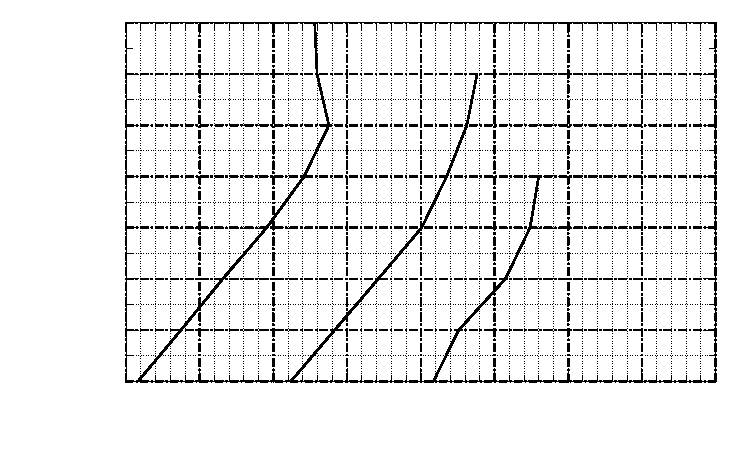
\includegraphics{../graphs/cruise_speed}}%
    \gplfronttext
  \end{picture}%
\endgroup
